\documentclass[../main.tex]{subfiles}

\begin{document}
\chapter{Lecture 3 - 16-03-2020}
Data point x represented as sequences of measurement and we called this
measurements features or attributes.\\
$$ x = (x_1,..., x_d)  \qquad x_1 \quad \textit{feature value}
x \in X^d \qquad X = \barra{R}^d \qquad X = X_1 \cdot x \cdot ... \cdot X_d \cdot x
$$
\\
$
\textit{Label space } Y\\
\textit{Predictor } f : X \rightarrow Y \\
$
\\
Example $(x,y)$ \qquad y is the label associated with x\\
($ \rightarrow y$ is the correct label, the ground truth)\\
\\
Learning with example $(x_1,y_1)...(x_m,y_m)  \quad \textit{training set} $\\\\
Training set is a set of examples with every algorithm can learn.......\\\\
Learning algorithm take training set as input and produces a predictor as output.\\\\
\\
\begin{figure}[h]
    \centering
    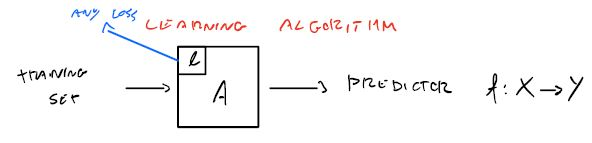
\includegraphics[width=0.8\linewidth]{../img/lez3-img1.JPG}
    \caption{Example of domain of $\knn$}
    %\label{fig:}
\end{figure}\\
\\With image recognition we use as measurement pixels.\\
How do we measure the power of a predictor?\\
A learning algorithm will look at training set, algorithm and generate the predictor. Now the problem is verify the score. \\
Now we can consider a test set collection of example
\\
$$ \textit{Test set} \qquad(x'_1, y'_1)...(x'_n,y'_n) $$
Typically we collect big dataset and then we split in training set and test set
randomly.\\
\textbf{Training and test are typically disjoint}
\\
How we measure the score of a predictor? We compute the average loss.\\
The error is the average loss in the element in the test set.\\
$$
\textit{Test error }\qquad \frac{1}{n}\cdot \sum_{t=1}^{n} \ell(f(x'_t),y')
$$
In order to simulate we collect the test set and take the average loss of the predictor of the test set. This will give us idea of how the.. \\
Proportion of test and train depends in how big the dataset is in general.
Our \textbf{Goal}: A learning algorithm ‘A’ must output f with a small test error.
A does not have access to the test set. (Test set is not part of input of A).\\
Now we can think in general on how a learning algorithm should be design.
We have a training set so algorithm can say:\\
\textbf{‘A’ may choose f based on performance on training set.}

$$
\textit{Training error }\qquad \hat{\ell}(f) = \frac{1}{m}\cdot \sum_{t=1}^{m} \ell(f(x_t),y_t)
$$
Given the training set $(x_1,...,x_m) (y_1,...,y_m)$
\\
If $\hat{\ell}(f)$ for same f, then test of f is also small
\\
Fix F set of predictors output $\hat{f}$\\
$$ \hat{f} = arg\,min\, \hat{\ell}(f)\\ f \in F $$
\\
\textbf{This algorithm is called Empirical Risk Minimiser (ERM)}
\\
When this strategy (ERM) fails?\\
ERM may fails if for the given training set there are:\\
Many $f \in F$ with small $\hat{\ell}(f)$, but not all of them have small test error
\\\\
There could be many predictor with small error but some of them may have big test error. Predictor with the smallest training error doesn’t mean we will
have the smallest test error.\\
I would like to pick $f^*$ such that:
$$ f^* = arg\,min \frac{1}{n} \cdot \sum_{t=1}^{m} \ell(f(x'_t),y_t) \\ \qquad f \in F $$
where $\ell(f(x'_t),y_t)$ is the test error
\\
ERM works if $f^* \textit{such that} \qquad f^* = arg\,min\, \hat{\ell}(f)\qquad f \in F$
\\
So minimising training and test????? Check videolecture\\
We can think of f as finite since we are working on a finite computer.\\
We want to see why this can happen and we want to formalise a model in
which we can avoid this to happen by design:
We want when we run ERM choosing a good predictor with ...... PD\\\\


\section{Overfitting}
We called this as overfitting: specific situation in which ‘A’ (where A is the
learning algorithm) overfits if f output by A tends to have a training error much
smaller than the test error.\\
A is not doing his job (outputting large test error) this happen because test
error is misleading.\\
Minimising training error doesn’t mean minimising test error. Overfitting is bad.\\
Why this happens?\\
This happen because we have \textbf{noise in the data}\\

\subsection{Noise in the data}

Noise in the data: $y_t$ is not deterministically associated with $x_i$.\\\\
Could be that datapoint appears more times in the same test set.
Same datapoint is repeated actually I’m mislead since training and dataset not
coincide.
Minimising the training error can take me away from the point that minimise
the test error.\\
Why this is the case?
\begin{itemize}
\item Some \textbf{human in the loop}: label assigned by people.(Like image contains
certain object but human are not objective and people may have different
opinion)
\item \textbf{Lack of information}: in weather prediction i want to predict weather error.
Weather is determined by a large complicated system. If i have humidity
today is difficult to say for sure that tomorrow will rain.
\end{itemize}
When data are not noise i should be ok.
\\
\textbf{Labels are not noisy}\\\\\\\\
Fix test set and trainign set.
$$ \exists f^* \in F \qquad y'_t = f^*(x'_t) \qquad \forall (x'_t,y'_t)\quad \textit{in test set} $$
$$ \qquad \qquad \qquad \qquad  y_t = f^+(x_t) \qquad \forall (x_t,y_t) \quad \textit{in training set} 
$$
\\
Think a problem in which we have 5 data points(vectors) :\\
$
\vec{x_1},...\vec{x_5} \qquad \textit{in some space X}
$
\\
We have a binary classification problem $Y = \{0,1\}$
\\
$
\{ \vec{x_1},..., \vec{x_5} \} \in X \qquad Y= \{0,1\}\\
$
\\ $F$ contains all possible calssifier $2^5 = 32 \qquad f: \{x_1,...,x_5\} \rightarrow \{0,1\}
$
\\\\
\begin{tabular}{ |p{2cm}||p{2cm}|p{2cm}|p{2cm}|p{2cm}|p{2cm}|  }
 \hline
 \multicolumn{6}{|c|}{Example} \\
 \hline
  & $x_1$ & $x_2$ & $x_3$ & $x_4$ & $x_5$ \\
 \hline
 f   &0     &0 &   0  & 0& 0 \\
 $f^{'}$  &0     &0 &   0  & 0& 1 \\
 $f^" $ &..     &..&   .. &..& .. \\

 \hline
\end{tabular}
\\\\
\[
\textit{Training set} \quad {x_1,x_2,x_3} \quad f^+
\\
\]
\[
\textit{Test set} \quad {x_4,x_5} \quad f^* 
\]
\\
$
4 \textit{ classifier } f \in F \qquad \textit{will have } \hat{\ell}(f) = 0
\\\\
	(x_1,0) \quad (x_2,1) \quad (x_3,0) \\
	(x_4,?) \quad (x_5, ?) \\
	f^*(x_4) \quad f^*(x_5)
$
\\
If not noise i will have deterministic data but in this example (worst case) we
get problem.\\
I have 32 classifier to choose: i need a larger training set since i can’t
distinguish predictor with small and larger training(?) error.
So overfitting noisy or can happen with no noisy but few point in the dataset to
define which predictor is good.\\



\section{Underfitting}
‘A’ underfits when f output by A has training error close to test error but they
are both large.\\
Close error test and training error is good but the are both large.
\\
$$
A \equiv ERM  \textit{, then A undefits if F is too small} \rightarrow \textit{not containing too much predictors}
$$
\\
In general, given a certain training set size:
\begin{itemize}
\item Overfitting when $|F|$ is too large (not enough points in training set)
\item Underfitting when $|F|$ is too small
\end{itemize}
Proportion predictors and training set
\\
$$
|F|, \textit{ i need } ln |F| \quad \textit{bits of info to uniquely determine } f^* \in  F
$$
$$
m >> ln |F| \qquad when \quad |F| < \infty \textit{\\ where m is the size of traning set}
$$
\\
\section{Nearest neighbour}
This is completely different from ERM and is one of the first learning
algorithm. This exploit the geometry of the data.
Assume that our data space X is:
\\
$ X \equiv \barra{R}^d \qquad x = (x_1, ..., x_d) \qquad y-\{-1,1\}
$
\\
S is the traning set $(x_1,y_1)...(x_m,y_m) \\ x_t \in \barra{R}^d \qquad y_t \in \{-1,1\} \\\\
d = 2 \rightarrow \textit{2-dimensional vector}\\
$\\
where + and - are labels
\newpage
\textbf{Point of test set}
\\
If i want to predict this point?
\begin{figure}[h]
    \centering
    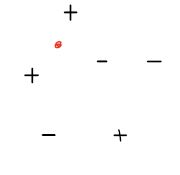
\includegraphics[width=0.4\linewidth]{../img/lez3-img2.JPG}
    \caption{Example of domain of $\knn$}
    %\label{fig:}
\end{figure}
\\
Maybe if point is close to point with label i know then. Maybe they have the same label.
\\
$\hat{y} = + \quad or \quad  \hat{y} = - $
\\\\
\begin{figure}[h]
    \centering
    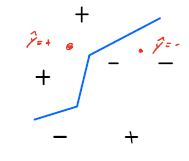
\includegraphics[width=0.4\linewidth]{../img/lez3-img3.JPG}
    \caption{Example of domain of $\knn$}
    %\label{fig:}
\end{figure}\\
\\
I can came up with some sort of classifier.
\\\\
Given $S$ training set, i can define $\hnn$  $X \rightarrow \{-1,1\}\\
$
$\hnn(x) = $ label $y_t$ of the point $x_t$ in $S$ closest to $X$\\
\textbf{(the breaking rule for ties)}
\\
For the closest we mean euclidian distance
\\
$ X = \barra{R}^d
\\
$
$$ 
\| x - x_t \| = \sqrt[] {\sum_{e=1}^{d} (x_e-x_t,e)^2}
$$\\
$$
\hat{\ell}(\hnn) = 0  
$$
$$
\hnn (x_t) = y_t
$$
\\
\textbf{training error is 0!}
\end{document}